\chapter{Sperimentazione e correzioni}
\label{sperimentazione}
\thispagestyle{empty}

%Si mostra il progetto dal punto di vista sperimentale, le cose materialmente realizzate. In questa sezione si mostrano le attivit\`a sperimentali svolte, si illustra il funzionamento del sistema (a grandi linee) e si spiegano i risultati ottenuti con la loro valutazione critica. Bisogna introdurre dati sulla complessit\`a degli algoritmi e valutare l'efficienza del sistema.

%discorso sulla fisica e di tutti i valori?

\section{Realizzazione del sistema}
Il sistema assemblato e impostato per il funzionamento si presenta come in figura.
 \begin{figure}[htb]
    \centering
    \vspace{-0.7cm}
    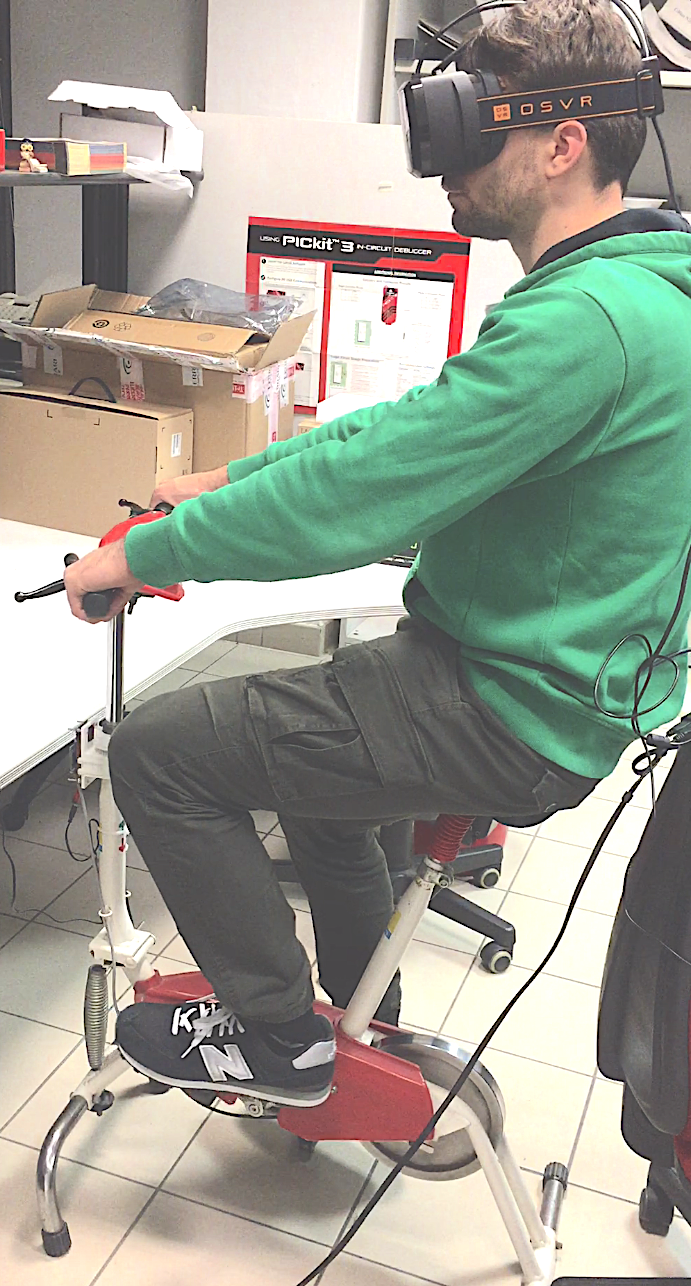
\includegraphics[height=11cm]{finale}
    \caption{Il sistema assemblato\label{fig:finale}}
    %\vspace{-0.3cm}
\end{figure}
\newpage
\noindent Per avere un corretto funzionamento di tutto il sistema è necessario seguire obbligatoriamente una determinata serie di operazioni nell'esatto ordine:
\begin{itemize}
  \item il computer principale deve essere accesso, deve avere il ricevitore bluetooth collegato e deve avere il progetto di Unity già pronto per essere avviato
  \item collegare alla corrente il microcontrollore della cyclette
  \item prendere l'hub dell'OSVR e collegarlo alla corrente
  \item collegare il visore all'hub
  \item prendere il cavo HDMI-USB dell'OSVR e collegare HDMI e USB all'hub
  \item collegare l'usb al computer
  \item collegare l'HDMI al computer
  \item eseguire il server OSVR nel computer
  \item far partire l'applicazione premendo il tasto \textit{play} su Unity.
  \item una volta partito, è necessario spostare la schermata \textit{game} nel monitor virtuale a destra, poiché l'OSVR viene rilevato dal computer come un monitor.
  \item a questo punto è possibile indossare il visore e cominciare ad utilizzare la bicicletta.
\end{itemize}

\newpage
\section{OSVR e le impostazioni iniziali}
\noindent Nei primi test eseguiti con l'OSVR appena installato, si è riscontrato un bug che, all'avviamento della simulazione, posizionava la telecamera ruotata di 90\degree verso destra e un inversione di rotazione tra roll (su Z) e pitch (su Y). La chiarificazione di questi movimenti si ha in figura \ref{fig:headmov}.
\begin{figure}[htb]
    \centering
    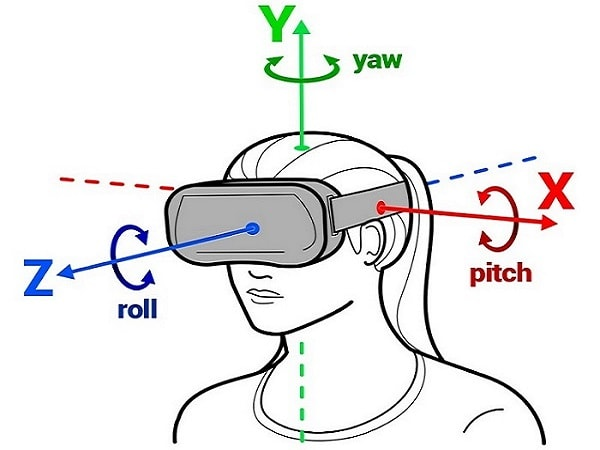
\includegraphics[height=8cm]{headmov}
    \caption{Le varie rotazioni della testa\label{fig:headmov}}
    \vspace{-0.3cm}
\end{figure}
\noindent Il problema è che l'OSVR necessita di una calibrazione iniziale che non era stata eseguita dopo l'installazione. Inizialmente si è risolto il problema posizionando la bicicletta a (0,0,0) con l'oggetto \textit{VRDisplayTracked} interno alla bicicletta con posizione (0,0,0) e tutte le rotazioni a 0. In questo modo le rotazioni a tempo di esecuzione erano tutte corrette. Tuttavia, esiste un tool fornito dal portale di sviluppo di OSVR che permette di resettare il sistema di coordinamento del visore, chiamato \textit{OSVRResetYaw}. Lanciando l'eseguibile di questo tool, è possibile resettare la posizione e le rotazioni del visore, portandolo ai valori impostati su Unity.

\section{Calibrazioni della fisica virtuale}
Testando la bicicletta nel tracciato di gara citato nella sottosezione \nameref{ambientazione} a pagina \pageref{ambientazione} si sono potuti definire al meglio i valori della fisica del mondo virtuale. I problemi principali erano: la velocità da fornire dopo una pedalata, l'inerzia e la frenata in caso di pedalata nulla. 
%Oltre a questi problemi principali è stata anche gestita la limitazione dello sterzo in caso di elevata velocità per evitare di perdere il controllo della bicicletta.

\subsection{Velocità}
La velocità è stata limitata al valore \textit{40} che rappresenta una velocità poco superiore alla realtà, ma rende realistico il modo in cui la bicicletta si muove nel mondo virtuale. Il valore \textit{MaxSpeedPedalata} è stato impostato a 20 e rappresenta, in modo inversamente proporzionale, quanto una pedalata può influire sulla velocità: più piccolo è, maggiore sarà l'accelerazione che ne deriva. Il valore che principalmente influenza la velocità della bicicletta è \textit{Engine Torque}. Questo è stato impostato a 1500 per avere una buona accelerazione ad ogni pedalata, ma è stato raggiunto per tentativi. Sotto i 1000 si otteneva una scarsa accelerazione, mentre sopra i 3000 si otteneva una velocità non realista che portava la bicicletta a inpennarsi. Per evitare l'effetto impennata è stato spostato l'oggetto \textit{Bilanciamento} fino ad un punto in cui la bicicletta non si ribaltava neanche durante dei salti.
 \begin{figure}[htb]
    \centering
    %\vspace{-0.7cm}
    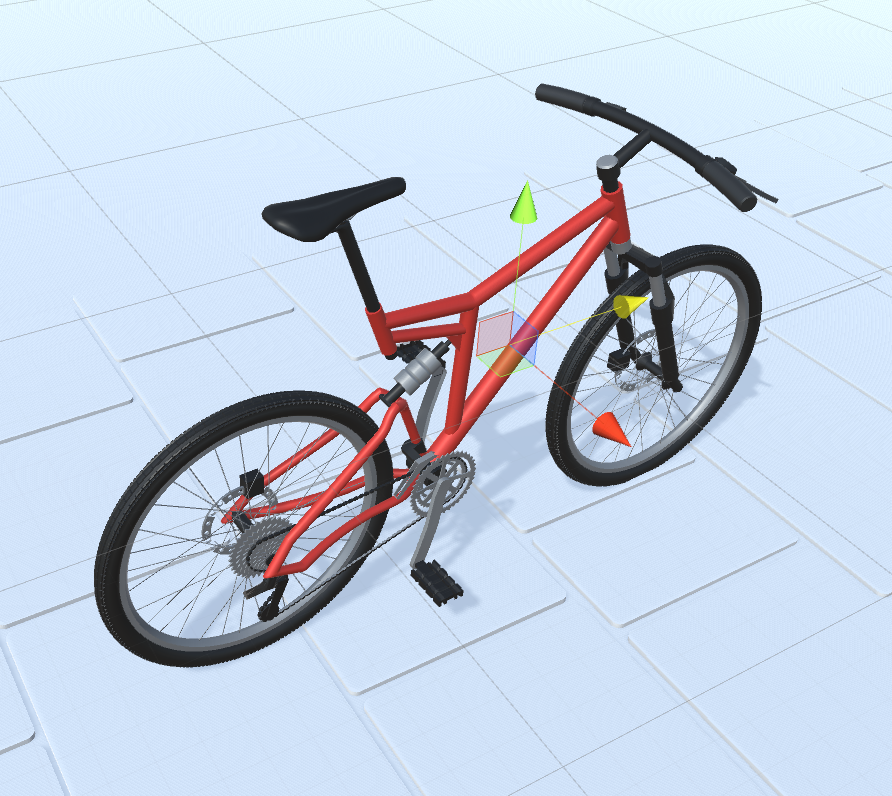
\includegraphics[height=8cm]{bilanciamento}
    \caption{Il punto in cui viene applicato il centro di massa\label{fig:bilanciamento}}
    %\vspace{-0.3cm}
\end{figure}

\subsection{Frenata e Inerzia}
I valori che influenzano la frenata sono \textit{Brake} e \textit{Friction}. Il primo è stato impostato a 2500 poiché con valori inferiori la bicicletta frena troppo lentamente e con valori superiori, faticava addirittura a partire. Il secondo è stato impostato a 6, poiché per valori molto superiori, la ruota posteriore slitta. Entrambi i valori sono stati impostati uno relativo all'altro durante la sperimentazione. L'inerzia viene gestita tramite questi valori nello script \texttt{MotoController} nella funzione \texttt{Braking}.

%\subsection{Sterzata}
%Per impedire che ad alte velocità






































%